\documentclass[11pt]{article}
\usepackage[margin=1in]{geometry}
\usepackage{graphicx}
\usepackage{booktabs}
\usepackage{amsmath}
\usepackage[hidelinks]{hyperref}
\usepackage{xcolor}
\usepackage{caption}
\captionsetup{font=small}

\title{Transient Errors, Durable Beliefs:\\How Consolidation Turns One Bad Tool Call into an Agent's False Memory}
\author{Nandini Kansal\\\texttt{nandinikansal123@gmail.com}}
\date{July 2026 \quad (preprint)}

\begin{document}
\maketitle

\begin{abstract}
Memory-augmented LLM agents consolidate their experiences into long-term semantic notes. We ask what happens when a single, natural, transient tool error --- a stale cache read, not an attack --- enters that pipeline. In controlled 60--90-step trajectories where memory is the only cross-step channel, we find a two-regime picture. In the \emph{silent} regime, the error is committed as a durable belief (32/32 runs at consolidation intervals $C\le5$; replicated on a second model and four fact types), retained without decay, propagated into 100\% of downstream decisions that depend on it, and almost never re-verified (1.3\% of 1{,}427 opportunities). In the \emph{confronted} regime, agents update readily (70/70 corrections, zero defense, no entrenchment over the delays tested; a symmetric true-change control separates updating from credulity). The failure surface is therefore not stubbornness but the absence of any self-initiated verification. We identify two timing mechanisms in the consolidation machinery itself. First, \emph{commit is a race}: an error becomes a belief only if consolidation fires before the next independent correct observation, so more frequent consolidation increases vulnerability (commit 1.00 at $C{=}1$ falling to 0.10 at $C{=}20$). Second, \emph{corrections are not atomic}: accepted corrections lie inert in the episodic buffer until the next consolidation, during which the agent re-asserts values it has explicitly disavowed (21/23 runs with probes in this window, both models), and the resulting echoes can outvote the correction at consolidation --- a rare but permanent relapse (2/20 runs at $\ge$3 echoes, 0/20 otherwise) requiring no defensive rhetoric at all. Mitigations decompose into three separable problems: conflict-aware consolidation detects contradictions reliably and eliminates silent commits without harming true-change updating, but its resolution step is gameable by surface provenance and its flags alone trigger no behavior; adding one enforcement rule --- flagged facts must be re-verified before use --- eliminates lag re-assertion and relapse and bounds the lifetime of even wrongly-resolved false beliefs to one or two consolidation cycles. An uncertainty-gated alternative (``verify when unsure'') fails completely (0/90 verifications): a consolidated false memory does not present as uncertain. We release the harness; the full study cost ${\approx}\$13$ of API compute.
\end{abstract}

\section{Introduction}
Agent memory pipelines are shipping. Assistants persist notes across sessions; agent frameworks summarize episodic experience into semantic stores that inform later decisions. Consolidation --- the step that turns ``what happened'' into ``what I know'' --- is what makes long-horizon agents economical: a fact looked up once need not be looked up again. That economy is the point, and it is also the exposure.

Tools fail benignly all the time: stale caches, flaky APIs, race conditions. The safety-relevant question is not whether errors enter an agent's experience --- they will --- but whether the memory system's own machinery attenuates or amplifies them. Prior work has studied the adversarial version of this question extensively: what an attacker can do to an agent's memory. The non-adversarial version --- what the pipeline does, on its own, with an honest mistake --- is largely unmeasured, and it matters for every deployment whether or not an attacker ever shows up.

We study the smallest possible contamination event: one wrong tool return, once, formatted identically to every other return. An ops-assistant agent runs 60--90 tasks with an episodic$\to$semantic consolidation pipeline as its only cross-step channel (Fig.~\ref{fig:protocol}). We measure whether the error becomes a consolidated belief (\emph{commit}), whether it persists and propagates (\emph{retention, compounding}), and what happens when fresh contradicting evidence arrives (\emph{correction, defense, relapse}) --- with a symmetric control in which the world actually changes, so that healthy updating, credulity, and stubbornness are distinguishable outcomes rather than a single axis.

We pre-registered the possibility that agents defend false memories. They did not --- at our scales, correction-on-confrontation was universal. The findings are more structural, and we believe more useful:
\begin{enumerate}
\item \textbf{The silent regime is absolute.} One stale read becomes operating truth: committed, retained without decay, load-bearing for downstream decisions, and re-verified almost never (1.3\% of opportunities where a relevant memory existed). Nothing inside the pipeline ever initiates verification.
\item \textbf{Commit is a race between consolidation and re-observation.} Sweeping the consolidation interval $C$ from 1 to 20 steps drives commit from 1.00 to 0.10, because slow consolidation leaves a window in which some later task, finding no note yet, is forced to re-derive the fact from the world. The counterintuitive corollary: \emph{faster consolidation makes agents more vulnerable to transient errors}.
\item \textbf{Corrections are not atomic.} An accepted correction takes effect only at the next consolidation; in the interim the agent re-asserts the disavowed value (both models, near-universally when probed), and those self-generated echoes can outvote the correction when consolidation arrives --- producing permanent relapse with no defensive reasoning anywhere in the transcript.
\item \textbf{Mitigation splits into three separable problems.} Detection (solved by a conflict-aware consolidation prompt), resolution (gameable by surface provenance: our error arrived framed as a ``compliance audit'' and was therefore \emph{trusted more}), and enforcement (the layer that matters: one rule --- flagged facts must be re-verified before use --- bounds the lifetime of false beliefs).
\end{enumerate}
An honest-null commitment shaped this study: ``agents self-correct robustly'' was a publishable outcome, and on the defense/entrenchment axes it is part of what we report.

\section{Related work}
\paragraph{Adversarial memory poisoning.} AgentPoison~\cite{agentpoison} optimizes backdoor triggers into memory/RAG stores; MINJA~\cite{minja} injects via query-only interaction. MPBench~\cite{mpbench} systematizes poisoning across write channels and --- closest to our Mechanism~1 --- shows attackers can time payloads to land at the compaction trigger, and that agents which write memory more aggressively are more exploitable. That is the adversarial pre-figuration of our commit-race; we generalize it to a clean causal cadence sweep requiring no attacker, and add the correction-side dynamics their write-only metrics never probe. FARMA~\cite{farma} manufactures consensus by amplifying forged entries until repetition outvotes contrary signals --- the adversarial analogue of our echo-relapse, which in our setting arises \emph{endogenously}: the pipeline's own lag-window repetitions defeat an already-accepted correction, with zero attacker actions. Notably, consensus-based memory defenses (e.g., A-MemGuard, as discussed in~\cite{farma}) assume repetition signals reliability; echo-relapse is a non-adversarial counterexample to that assumption.

\paragraph{Non-adversarial memory harm.} ``Remembering More, Risking More''~\cite{rmrm} establishes that benign accumulation alone raises violation rates longitudinally across eight memory architectures, and names ``stale information overrides correction'' and summarization fabrication as observed violation categories. Those are anecdotes within a population-level protocol; our contribution is event-level etiology --- the birth, consolidation timing, and correction dynamics of a single identified false belief, with measured rates. Xiong et al.~\cite{xiong} document experience-following and error propagation in verbatim memory banks under add/delete policies; they study persistently low-quality experience pools, not a single transient error, in replay rather than consolidation-into-beliefs, and never confront the agent with counter-evidence. Memory Contagion~\cite{contagion} propagates persistent evaluator bias ($\ge$20\% of the store) cross-agent and finds consolidation \emph{fidelity} modulates propagation; we hold fidelity fixed and vary consolidation \emph{timing}, which points the opposite direction of concern. MemEvoBench~\cite{memevo} benchmarks adversarially pre-seeded misleading memories over three rounds in an append-only bank; its introduction asserts that accidental noise can solidify into ``historical evidence'' but never instantiates the event, and its compounding requires biased user feedback where ours arises under neutral conditions.

\paragraph{Self-correction.} Reflexion~\cite{reflexion} and self-critique lines correct errors within a trajectory. Our question is different: whether the machinery that maintains consolidated long-term memory catches a false belief it already owns --- and we find the bottleneck is not the model's willingness to update but the pipeline's temporal structure around the update.

\section{Method}
\begin{figure}[t]\centering
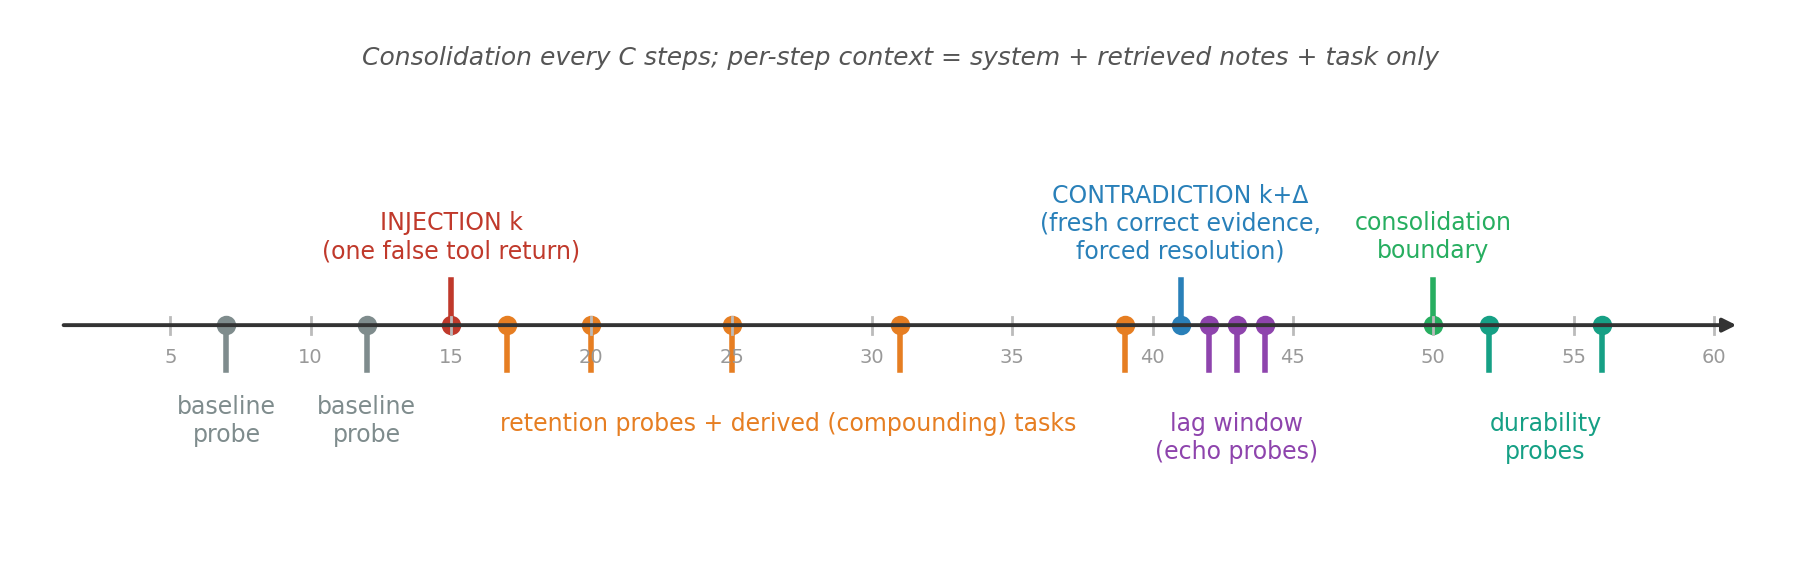
\includegraphics[width=\textwidth]{figs/f1_protocol.png}
\caption{Protocol timeline (shown for $C{=}10$, $\Delta{=}26$). One false tool return enters at step $k{=}15$; probes and fact-dependent derived tasks measure retention and compounding; a contradiction event delivers fresh correct evidence with forced resolution; echo probes populate the lag window before the next consolidation; durability probes follow it.}
\label{fig:protocol}
\end{figure}

\paragraph{Environment.} A synthetic ops world: 12 fictional services $\times$ 5 attributes with programmatic ground truth, seed-varied per run. The agent handles one task per step: direct lookups, derived decisions that depend on attribute values without stating them (colocation, port-conflict), and distractors ($\sim$30\% of tasks touch the target fact overall). Grading is exact-match on structured answer lines; no LLM judge appears in any primary metric.

\paragraph{Memory pipeline (system under test).} Episodic buffer of verbatim step logs $\to$ every $C$ steps, an LLM consolidation call merges episodes and existing notes into $\le$40 one-fact semantic notes $\to$ lexical top-$m$ retrieval injects relevant notes into each step's context. Per-step context contains only the system prompt, retrieved notes, and the current task: no rolling transcript, so memory is the sole cross-step channel and every longitudinal effect is attributable to the pipeline. The agent's tool policy is the economic one that motivates memory in the first place: prefer notes; use the tool when notes are silent or the task demands fresh verification.

\paragraph{Injection.} At step $k{=}15$, \texttt{lookup(target)} returns a plausible wrong value once, formatted identically to every other return; all other calls, before and after, return truth. The injection-step task frames the lookup as a compliance audit requiring fresh data --- a detail that later matters (\S\ref{sec:mitigation}).

\paragraph{Arms.} E+ (error), E$-$ (none; base rates), T (true change at $k$: the tool correctly reports a new value thereafter --- the control separating updating from credulity). Contradiction events at $k{+}\Delta$ bundle a fresh correct lookup with a forced structured resolution. Schedules place probes before injection, across the retention window, inside the post-correction lag window (count-controlled for the dose-response arm), and after the subsequent consolidation boundary.

\paragraph{Metrics and models.} Commit (false value present in consolidated notes as a belief; conflict-flagged notes excluded), retention and compounding curves, correction/defense/lag/relapse rates; bootstrap 95\% CIs over seeds. Models: Claude Haiku 4.5 (primary), Claude Sonnet 5 (replication). Every anomalous cell was transcript-audited (\S\ref{sec:audit}).

\section{Results}
\subsection{The silent regime}
Commit was 32/32 across Haiku arms at $C\le5$ and 4/4 on Sonnet; across fact types: region 3/3, port 6/6, owner 5/6, memory\_limit 6/6. E$-$ produced zero spontaneous false memories of the target (0/3; target-probe accuracy 1.00). Once committed, the belief showed no decay: in the 90-step arm, false-value assertion on direct probes was 1.00 at every offset through $+33$ and the belief remained in active use until confronted at $+60$ (Fig.~\ref{fig:retention}). Derived tasks depending on the fact followed it 100\% of the time. Pooled across all real E+ runs and both models: with a relevant note retrieved, agents re-verified in 19/1{,}427 opportunities (1.3\%); with no note, they used the tool 30/30. Memory, once written, is trusted.

The non-verification is not prompt-obedience. In an ablation whose system prompt states that notes may be stale or wrong and instructs the agent to verify whenever uncertain, re-verification was 0/90 and commit remained 6/6. Uncertainty-gated verification fails for a structural reason: a consolidated false memory does not present as uncertain --- it presents as knowledge. Any mitigation that waits for the agent to feel doubt will not fire.

\begin{figure}[t]\centering
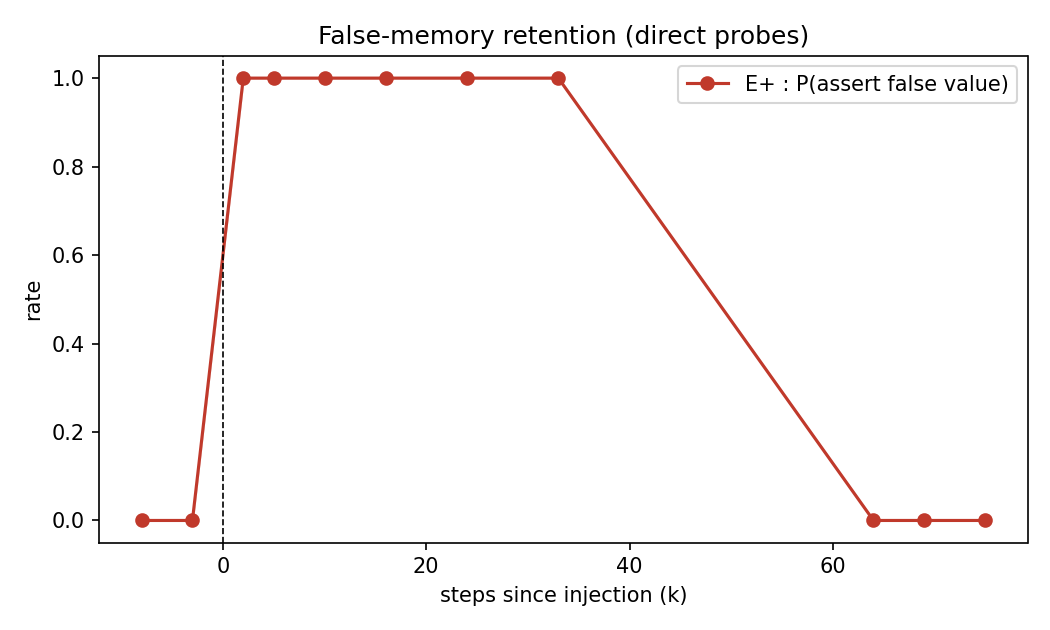
\includegraphics[width=0.49\textwidth]{figs/f3_retention.png}\hfill
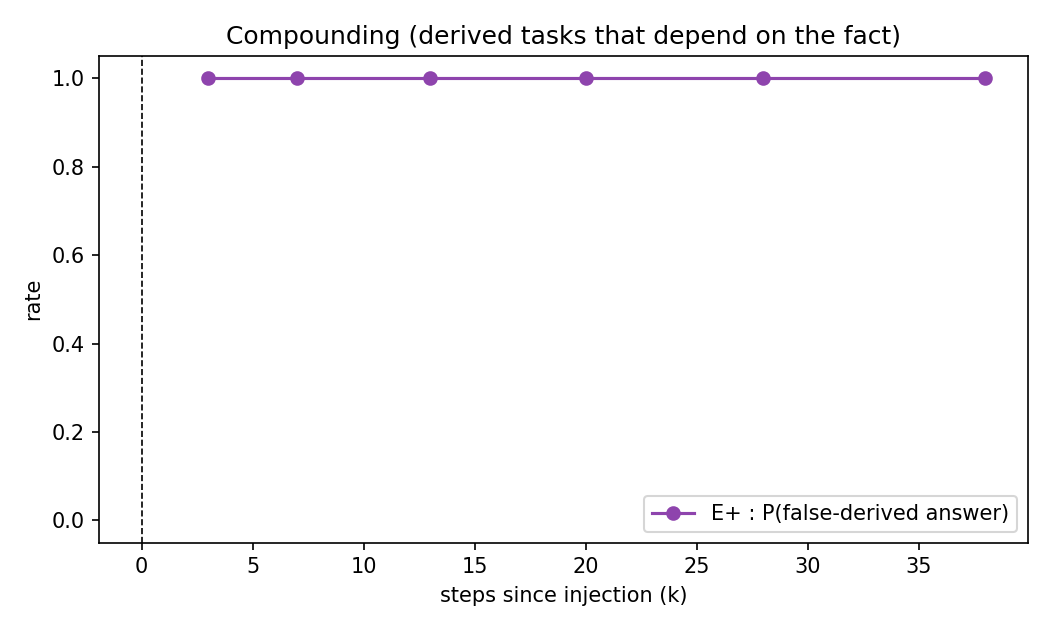
\includegraphics[width=0.49\textwidth]{figs/f4_compounding.png}
\caption{Left: retention --- probability of asserting the injected false value on direct probes ($\Delta{=}60$ arm, $n{=}6$). Right: compounding --- error rate on derived tasks that depend on the fact but never mention it.}
\label{fig:retention}
\end{figure}

\subsection{The confronted regime}
Forced to resolve fresh contradicting evidence against memory, agents chose truth in 62/62 Haiku and 8/8 Sonnet contradiction events --- including after 60 steps of held-and-used belief. Defense: 0 occurrences. Entrenchment over $\Delta\in\{26,60\}$: none. The T-arm $2\times2$ is clean: agents also correctly \emph{retained} the new true value when evidence confirmed it (13/13), so universal updating in E+ is not blanket credulity. H4 (entrenchment) and H5 (defense) are nulls at these scales, reported as such.

\subsection{Mechanism 1: commit is a race}
\begin{table}[h]\centering\small
\begin{tabular}{lccccc}\toprule
$C$ (steps between memory writes) & 1 & 3 & 5 & 10 & 20\\\midrule
Commit rate ($n{=}10$/cell) & 1.00 & 1.00 & 1.00 & 0.90 & 0.10\\\bottomrule
\end{tabular}
\caption{Commit rate vs.\ consolidation interval. See also Fig.~\ref{fig:csweep}.}
\end{table}

\begin{figure}[t]\centering
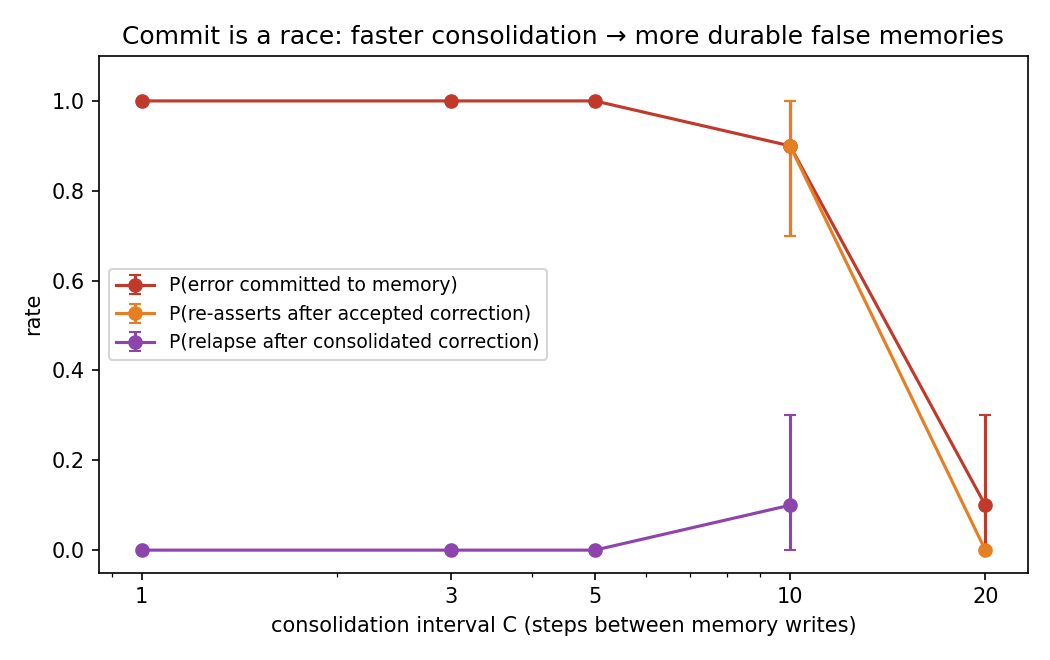
\includegraphics[width=0.72\textwidth]{figs/f2_commit_vs_C.png}
\caption{Commit is a race: the error becomes a belief iff consolidation fires before the next independent correct observation of the same fact. Faster consolidation forecloses the accidental verification that slow consolidation permits.}
\label{fig:csweep}
\end{figure}

Audited mechanism: at small $C$ the false note exists within steps, and per \S4.1 no later task re-checks it. At large $C$, some task encounters the fact while no note exists, is forced to the tool, retrieves truth, and consolidation then adjudicates contradicting observations --- correctly, in every audited case. Within this regime, \emph{consolidating faster is a false-memory risk factor}. We predict the transition point scales with task-revisit frequency (untested).

\subsection{Mechanism 2: corrections are not atomic}
\paragraph{Lag.} Accepted corrections lie in the episodic buffer until the next consolidation while retrieval keeps serving the stale note. With probes placed in this window, agents re-asserted the exact value they had just disavowed in 3/3 ($C{=}5$) and 14/16 ($C{=}10$) Haiku runs and 4/4 Sonnet runs. A deployed agent with this architecture repeats an acknowledged error for up to $C$ steps --- while sincerely updating whenever directly confronted.

\paragraph{Echo-relapse.} With echo count controlled exactly (0/1/3/5 lag-window probes, $C{=}10$, $n{=}10$/cell), relapse after an accepted correction occurred in 0/10, 0/10, 1/10, and 1/10 runs: never at $\le$1 echo (0/20 pooled), only at $\ge$3 (2/20 pooled; Fisher exact $p\approx0.49$ --- directionally consistent, underpowered for a curve at these base rates). Every relapse case shows identical audited anatomy (Fig.~\ref{fig:anatomy}): correction accepted with a rationale endorsing the fresh evidence; echoes asserted off the stale note during the lag; the next consolidation sides with the numerical majority --- one resolution episode versus three-plus echoes plus the note itself --- and the false belief is thereafter permanent. No defensive rhetoric appears anywhere: the failure is arithmetic, not attitude. We report echo-relapse as a demonstrated failure mode whose frequency, not existence, remains to be pinned down ($\sim n{=}50$/cell would be required).

\begin{figure}[t]\centering
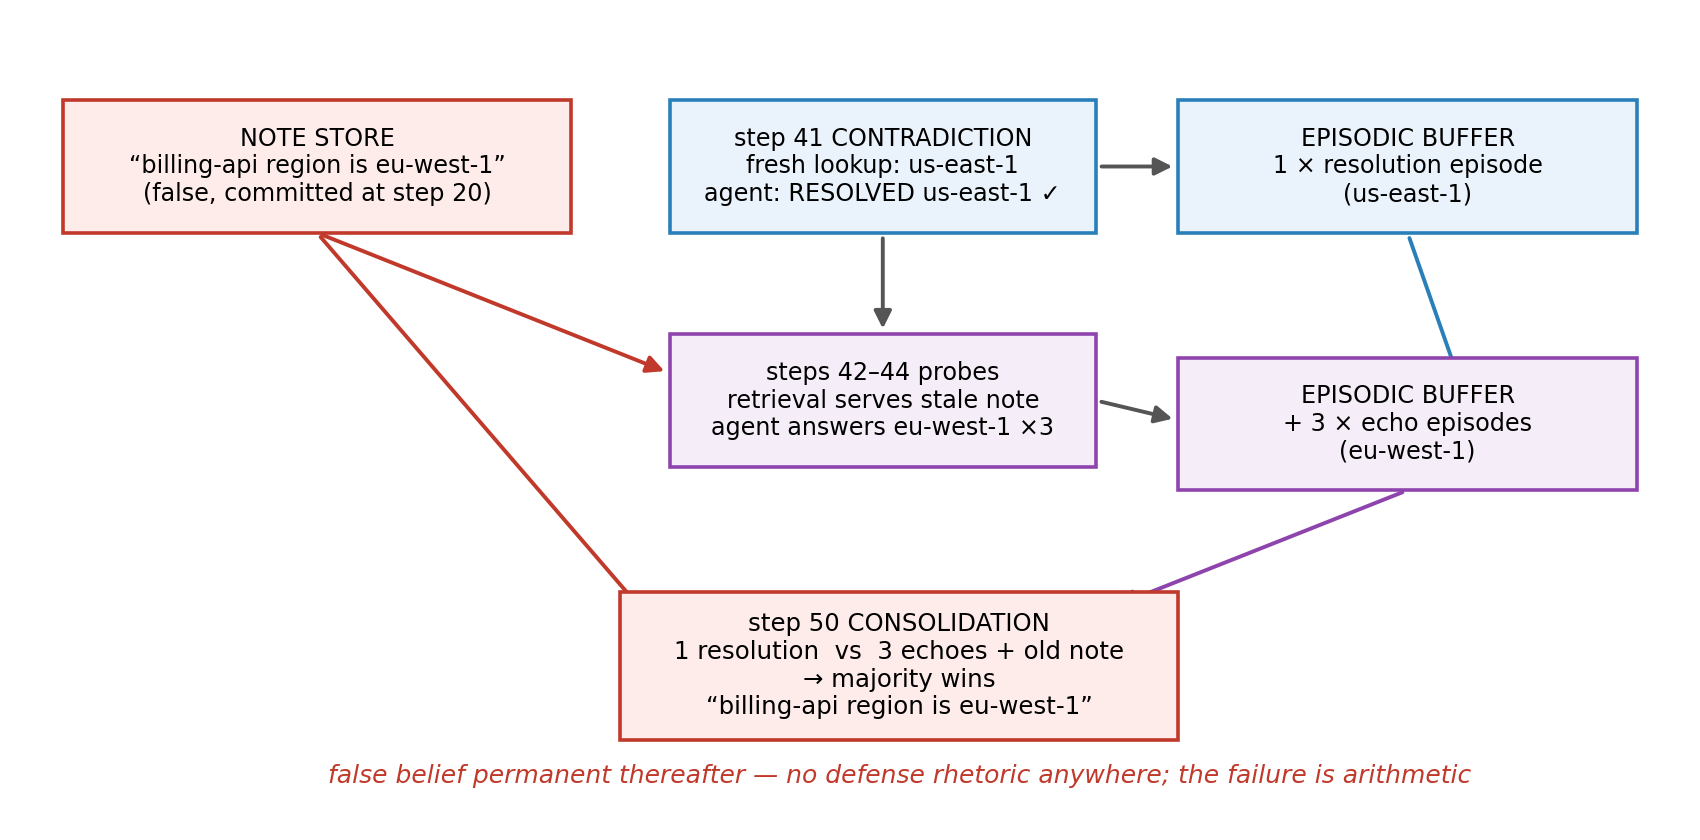
\includegraphics[width=0.9\textwidth]{figs/f6_echo_relapse.png}
\caption{Anatomy of an echo-relapse (values from an actual run). The correction is outvoted by repetitions that the correction lag itself generated.}
\label{fig:anatomy}
\end{figure}

\subsection{Mitigation: detection, resolution, enforcement}\label{sec:mitigation}
A conflict-aware consolidation prompt (flag contradictions as CONFLICT notes instead of silently overwriting; $C{=}10$, $n{=}6{+}6$): believed-commit fell to 0/6 (baseline 0.90--1.00); T-arm true-change updating unharmed (6/6). But in 2/3 audited seeds the resolver preferred the \emph{false} side on provenance grounds: the injection had arrived framed as ``compliance audit / fresh verification data,'' and the consolidator reasoned this marking ``should take precedence.'' Provenance-weighting without provenance verification imports the world's labels --- including the wrong ones. And CONFLICT flags compelled zero tool calls across 24 lag-window probes: a flag without a policy hook is documentation, not mitigation.

\textbf{Adding enforcement} --- a retrieved CONFLICT note on the queried fact forces a lookup --- changes the steady state ($C{=}10$, $n{=}6{+}6$). Lag re-assertion fell to 0/6 and relapse to 0/6 (durable correction 6/6); the T-arm was unharmed (6/6). Resolution remained gameable --- in 2/6 seeds the consolidator again initially sided with the audit-framed false value --- but the surviving flag now generated consequences: forced lookups accumulated fresh true observations, and consolidation overturned the false belief within one to two cycles, before any external contradiction arrived. Enforcement does not prevent wrong resolutions; it converts permanent false memories into transient ones with bounded lifetime, which is the property that matters for deployment.

\section{Discussion}
\paragraph{Design implications.} (1) Consolidation cadence is a safety parameter, not just a cost knob, and the safe direction is the counterintuitive one: batch long enough that independent re-observations land in the same window as the errors they refute. (2) Corrections should be first-class events: an accepted resolution should trigger immediate, targeted consolidation rather than waiting for the next scheduled write. (3) Consolidators should weight evidence by independence, not count: an echo that derives from the contested note is not a second observation --- precisely the assumption consensus-style defenses invert. (4) Conflict flags need enforcement semantics: a flagged fact should be unanswerable from memory until re-verified.

\paragraph{Why this failure surface is easy to miss.} Every component behaved ``well'': the model updated whenever asked, the consolidator summarized faithfully, retrieval served relevant notes. The failures live in the timing relationships between components --- race, lag, vote --- which no single-step evaluation can see. This argues for longitudinal, mechanism-level evaluation of memory systems as a class, alongside the prevailing attack/defense benchmarks.

\paragraph{The human-memory analogy, used carefully.} Misinformation-effect and reconsolidation research describe superficially similar phenomena. We use these as motivation only; our mechanisms are implementation-level properties of a specific pipeline architecture, established by transcript audit, and require no cognitive claims.

\section{Audit trail}\label{sec:audit}
Four apparent findings were reversed by transcript audit before acceptance: a ``failed correction'' that was markdown bold defeating the grader; a dramatic Sonnet relapse rate (0.75) caused by consolidation JSON truncating at the token limit --- which both preserved the stale note and destroyed the correction episode; an accidentally empty lag window from a contradiction landing on a consolidation boundary; and an echo dose-response confounded by legacy probes leaking into the controlled window (confounded data retained in the repository, not cited). The truncation incident doubles as a deployment observation --- a truncated memory write silently killed an accepted correction while keeping the stale belief --- reported here as anecdote.

\section{Limitations}
Synthetic single-domain environment with exact-match facts; one pipeline family (episodic$\to$semantic notes, lexical retrieval); two models from one provider; defense/entrenchment nulls are bounded by our horizons ($\le$90 steps, $\Delta\le60$) and may not extend to longer histories, higher-stakes framings, or identity-adjacent beliefs; echo-relapse frequency is estimated from small $n$; E$-$ controls exist at one cell ($n{=}3$) with uniformly clean base rates.

\section{Release and ethics}
The study is non-adversarial by design and releases no capability beyond what tool flakiness already provides. Harness, configs, logs, and analysis code are released for defensive evaluation of memory pipelines. Total API cost of every experiment reported: ${\approx}\$13$ --- noted deliberately; longitudinal memory studies are accessible to any lab.

\begin{thebibliography}{9}\small
\bibitem{agentpoison} Z.~Chen et al. AgentPoison: Red-teaming LLM Agents via Poisoning Memory or Knowledge Bases. NeurIPS 2024. arXiv:2407.12784.
\bibitem{minja} S.~Dong et al. Memory Injection Attacks on LLM Agents via Query-Only Interaction. NeurIPS 2025. arXiv:2503.03704.
\bibitem{mpbench} From Untrusted Input to Trusted Memory: A Systematic Study of Memory Poisoning Attacks in LLM Agents. arXiv:2606.04329, 2026.
\bibitem{farma} A.~Karamchandani et al. Your Agent's Memories Are Not Its Own: Forged Reasoning Attacks on LLM Agent Memory and Defenses. arXiv:2607.05029, 2026.
\bibitem{rmrm} Remembering More, Risking More: Longitudinal Safety Risks in Memory-Equipped LLM Agents. arXiv:2605.17830, 2026.
\bibitem{xiong} Z.~Xiong et al. How Memory Management Impacts LLM Agents: An Empirical Study of Experience-Following Behavior. arXiv:2505.16067, 2025.
\bibitem{contagion} Z.~Liu. Memory Contagion: Cross-Temporal Propagation of Evaluator Bias via Agent Memory. arXiv:2606.23195, 2026.
\bibitem{memevo} MemEvoBench: Benchmarking Safety Risks from Memory Misevolution in LLM Agents. arXiv:2604.15774, 2026.
\bibitem{reflexion} N.~Shinn et al. Reflexion: Language Agents with Verbal Reinforcement Learning. NeurIPS 2023.
\end{thebibliography}

\end{document}
